%versi 2 (8-10-2016) 
\chapter{Pendahuluan}
\label{chap:intro}
   
\section{Latar Belakang}
\label{sec:label}

Tugas merupakan suatu bentuk pembelajaran dan penilaian yang diberikan oleh pengajar kepada pelajar untuk membantu pelajar mendalami materi yang sudah diberikan\cite{prihatini:16:plagiarisme}. Pembagian tugas yang diberikan dapat dibagi menjadi 2 jenis yakni tugas individu dan tugas kelompok. Tugas individu merupakan tugas yang hanya ditanggung oleh satu individu. Sedangkan tugas kelompok merupakan tugas yang ditanggung oleh beberapa individu. Tugas yang telah diterima selanjutnya akan dikumpulkan kepada pengajar dan diberikan penilaian berdasarkan tingkat ketepatan jawaban dari tugas tersebut. Pengumpulan dan pengecekan tugas terutama \textit{coding} secara manual memiliki kekurangan dimana diperlukan banyak langkah dalam melakukan pengecekan dan pengiriman nilai. Selain itu, pengecekan secara manual juga terdapat kekurangan yakni kesulitan dalam menentukan pengecekan plagiarisme antara tugas pelajar. Oleh karena itu, dibutuhkan perangkat lunak untuk melakukan pengecekan secara otomatis salah satunya adalah \textit{Online Judge}.

\textit{Online Judge} merupakan sebuah perangkat lunak yang dapat melakukan pengecekan program sesuai dengan standar yang sudah diberikan. Perangkat lunak dapat menerima jawaban dari pelajar dan melakukan pengecekan secara otomatis. Perangkat lunak selanjutnya memberikan keluaran berupa nilai dari pelajar tersebut\cite{kurnia:01:judge}. Salah satu perangkat lunak \textit{Online Judge} terdapat pada prodi Informatika Universitas Katolik Parahyangan bernama \textit{SharIF Judge}. Gambar \ref{fig:judgeawal} menunjukan tampilan perangkat lunak \textit{SharIF Judge} yang terletak pada Universitas Katolik Parahyangan.

\begin{figure}[H]
	\centering  
	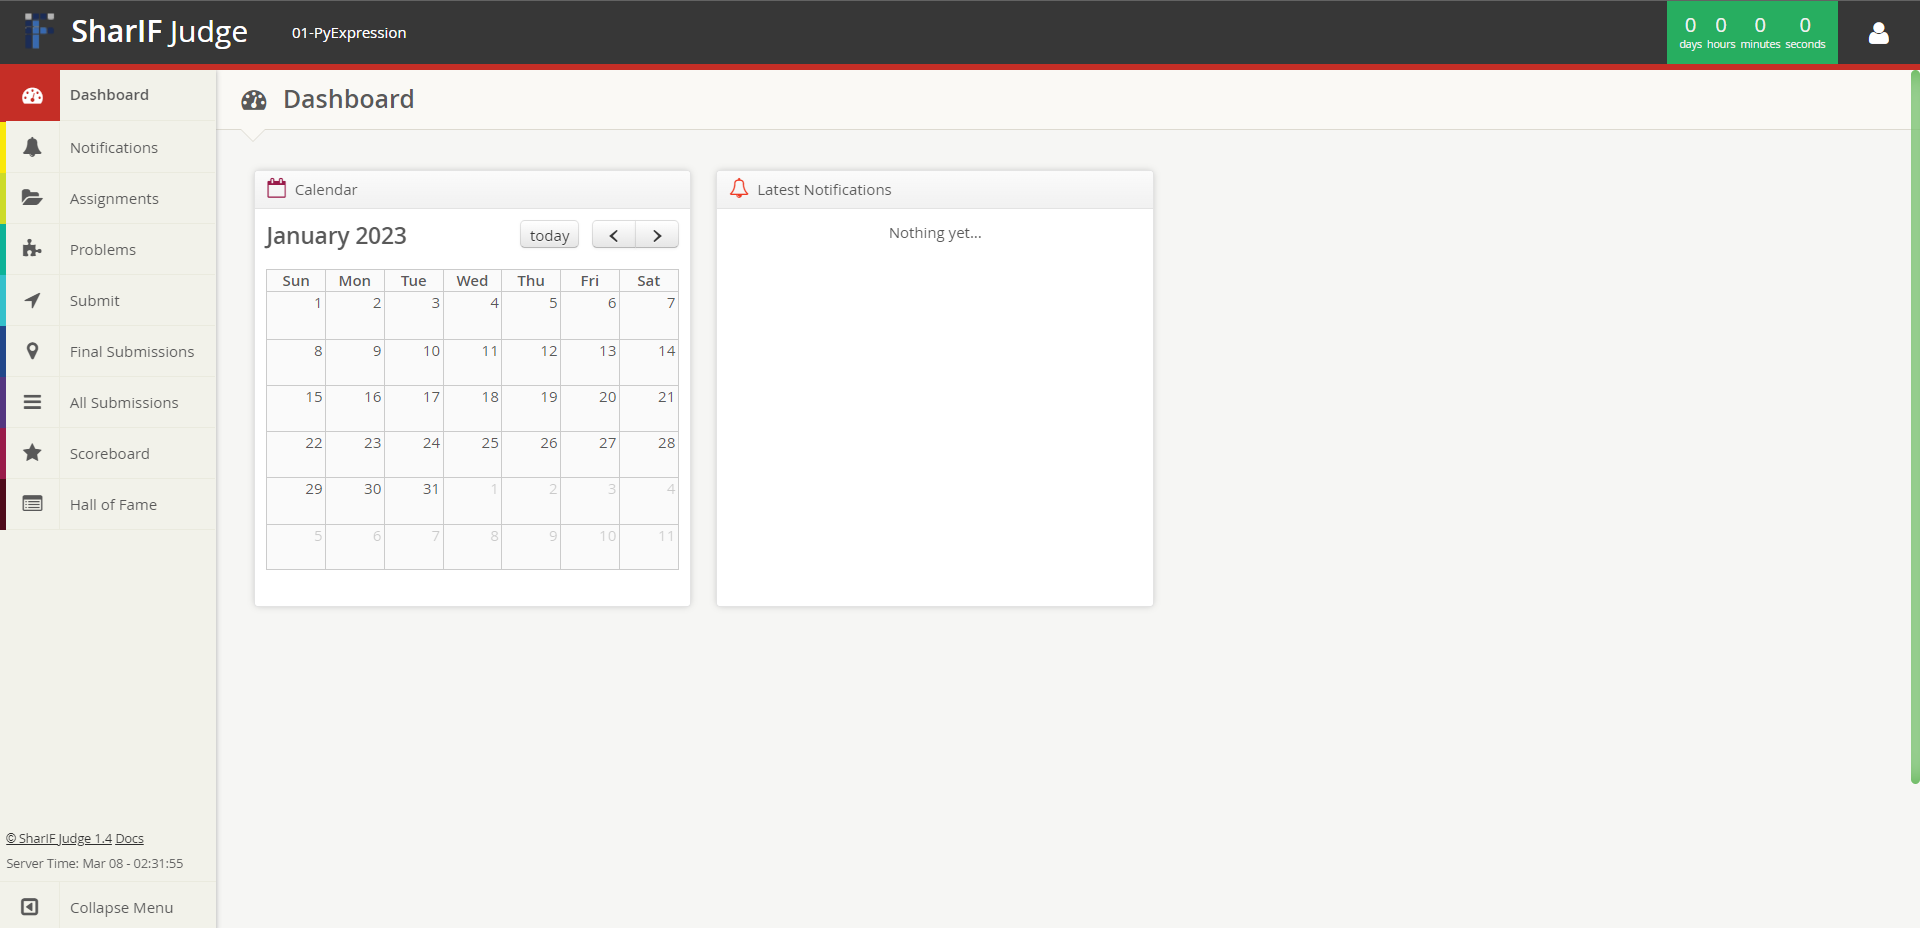
\includegraphics[scale=0.3]{judgeawal}  
	\caption[Tampilan halaman \textit{SharIF Judge}]{Tampilan halaman \textit{SharIF Judge}} 
	\label{fig:judgeawal} 
\end{figure} 


\textit{SharIF Judge} pada awalnya bernama \textit{Sharif Judge} yang merupakan sebuah perangkat lunak \textit{open source}. \textit{Sharif Judge} berfungsi untuk menilai kode dengan beberapa bahasa seperti C, C++, Java, dan Python secara online. \textit{Sharif Judge} pada awalnya dibentuk oleh Mohammad Javad menggunakan \textit{framework} \textit{CodeIgniter 3} yang merupakan \textit{framework} berbasis PHP atau \textit{Hypertext Preprocessor}. \textit{Sharif Judge} kemudian di \textit{fork} dan dimodifikasi menjadi \textit{SharIF Judge} dengan penambahan fungsi sesuai kebutuhan Informatika UNPAR untuk mengumpulkan tugas dan ujian mahasiswa. \textit{SharIF Judge} menggunakan autentikasi \textit{Remote Authentication Dial In Service} (RADIUS) dan \textit{Light Weight Directory Protocol} (LDAP) yang memungkinkan autentikasi menuju \textit{database} pusat pada RADIUS dan direktori pada LDAP. Autentikasi ini membutuhkan \textit{server} yang terintegrasi untuk menyimpan data-data yang diperlukan.

\textit{CodeIgniter 3} merupakan sebuah \textit{framework opensource} yang bertujuan untuk mempermudah dalam pembangunan sebuah aplikasi \textit{website} menggunakan PHP. \textit{CodeIgniter 3} menggunakan struktur MVC yang membagi \textit{file} menjadi 3 buah yaitu \textit{Model, View,} dan \textit{Controller}. Selain itu, \textit{CodeIgniter 3} merupakan \textit{framework} cepat karena hanya membutuhkan sedikit sumber daya untuk menjalankannya. \textit{Framework} ini juga menyediakan banyak \textit{library} untuk melakukan pembangunan\cite{ci3:22}. Namun, \textit{CodeIgniter} 3 sudah memasuki fase \textit{maintenance}\footnote{Pemberitahuan fase \textit{maintenance CodeIgniter 3} \url{https://codeigniter.com/download}(19 Maret 2023)} sehingga tidak mendapatkan pembaharuan lebih lanjut dari pembentuknya. \textit{CodeIgniter 3} pada akhirnya tidak dapat digunakan kembali dan kehilangan dokumentasi dari situs web resminya. Sehingga, perangkat lunak yang menggunakan \textit{CodeIgniter 3} perlu dikonversi ke \textit{framework} \textit{CodeIgniter} dengan versi terbaru yakni \textit{CodeIgniter 4}.

\textit{CodeIgniter 4} merupakan versi terbaru dari \textit{framework} \textit{CodeIgniter} yang memiliki banyak perubahan fitur dari versi sebelumnya. \textit{CodeIgniter 4} bisa dijalankan menggunakan versi PHP 7.4 atau lebih baru sedangkan \textit{CodeIgniter 3} bisa dijalankan menggunakan versi PHP 5.6 atau lebih baru. \textit{CodeIgniter 4} membagi \textit{file} menggunakan struktur MVC, namun memiliki struktur direktori berbeda dengan versi sebelumnya\cite{codeigniter:23:ci4}. Perubahan direktori ditunjukan oleh Gambar \ref{fig:dirMappingBab1}.
\begin{figure}[H]
	\centering  
	
\includegraphics[scale=0.5]{ci3ci4}  
	\caption[\textit{Pemindahan struktur aplikasi menuju \textit{CodeIgniter 4}}]{\textit{Pemindahan struktur aplikasi menuju \textit{CodeIgniter 4}}} 
	\label{fig:dirMappingBab1} 
\end{figure}

Gambar \ref{fig:dirMappingBab1} menunjukan perubahan struktur yang terdapat pada \textit{CodeIgniter 4}. Rincian perubahan dapat dilihat pada bab \ref{chap:analisis}. Pada tugas akhir ini dilakukan konversi \textit{SharIF Judge} dari \textit{CodeIgniter 3} menjadi \textit{CodeIgniter 4}. Konversi dilakukan agar \textit{SharIF Judge} dapat digunakan kembali apabila \textit{CodeIgniter 3} sudah tidak mendapat dukungan.

\section{Rumusan Masalah}
\label{sec:rumusan}
\begin{itemize}
	\item Bagaimana cara melakukan konversi \textit{SharIF Judge} pada \textit{CodeIgniter 3} menjadi \textit{CodeIgniter 4}? 
		\item Bagaimana cara menguji \textit{SharIF Judge} berbasis \textit{CodeIgniter 4}?.
\end{itemize}
\section{Tujuan}
\label{sec:tujuan}
Tujuan dari tugas akhir ini adalah sebagai berikut:
\begin{itemize}
	\item Melakukan konversi dengan megubah kode sesuai dengan standar \textit{CodeIgniter 4}.
	\item Melakukan pengujian dan perbandingan setiap fitur pada \textit{SharIF Judge} berbasis \textit{CodeIgniter 3} dengan \textit{SharIF Judge} berbasis \textit{CodeIgniter 4}.
\end{itemize}

\section{Batasan Masalah}
\label{sec:batasan}
Batasan masalah pada pembentukan tugas akhir ini adalah Autentikasi RADIUS dan LDAP tidak diuji karena tidak memiliki \textit{server} yang terintegrasi.

\section{Metodologi}
\label{sec:metlit}
Metodologi yang dilakukan dalam melakukan penelitian ini adalah sebagai berikut:
\begin{enumerate}
	\item Melakukan analisis dan eksplorasi fungsi-fungsi perangkat lunak \textit{SharIF Judge}.
	\item Melakukan studi literatur kebutuhan konversi dari \textit{CodeIgniter 3} menjadi \textit{CodeIgniter 4}.
	\item Melakukan konversi perangkat lunak dari \textit{CodeIgniter 3} menjadi \textit{CodeIgniter 4}.
	\item Melakukan pengujian dan eksperimen terhadap perangkat lunak yang sudah di konversi.
	\item Menyelesaikan pembentukan dokumen
\end{enumerate}

\section{Sistematika Pembahasan}
\label{sec:sispem}
Penelitian ini akan dibahas dalam enam bab yang masing-masing berisi:
\begin{enumerate}
	\item \textbf{Bab \ref{chap:intro}:} Pendahuluan
	
	Bab ini berisi latar belakang, rumusan masalah,tujuan, batasan masalah, metodologi, dan sistematika pembahasan.
	\item \textbf{Bab \ref{chap:teori}:} Landasan Teori
	
	Bab ini berisi pembahasan dasar-dasar teori yang akan digunakan dalam melakukan konversi \textit{SharIF Judge} dari \textit{CodeIgniter 3} ke \textit{CodeIgniter 4}. Landasan Teori yang digunakan diantaranya adalah \textit{SharIF Judge}, \textit{CodeIgniter 3}, \textit{CodeIgniter 4}, dan Konversi \textit{CodeIgniter 3} ke \textit{CodeIgniter 4}.
	\item \textbf{Bab \ref{chap:analisis}:} Analisis
	
	Bab ini berisi analisis \textit{SharIF Judge} dan analisis kebutuhan konversi menuju \textit{CodeIgniter 3}.
	\item \textbf{Bab \ref{chap:perancangan}:} Perancangan
	
	Bab ini berisi mengenai rancangan perangkat lunak yang akan dikonversi.
	\item \textbf{Bab \ref{chap:implementasidanpengujian}:} Implementasi dan Pengujian
	
	Bab ini berisi hasil implementasi dan pengujian yang telah dilakukan untuk melakukan konversi \textit{SharIF Judge} dari \textit{CodeIgniter 3} ke \textit{CodeIgniter 4}.
	\item \textbf{Bab \ref{chap:kesimpulandansaran}:} Kesimpulan dan Saran
	
	Bab ini berisi kesimpulan dari hasil konversi yang telah dilakukan dan saran-saran terhadap perangkat lunak.
\end{enumerate}
